%************************************************
\chapter[Abstracting the robot]{Abstracting the robot}\label{ch:capabilities}
%************************************************

\begin{flushright}{\slshape The essence of abstractions is preserving information that is relevant in a given context, and forgetting information that is irrelevant in that context.} \\ \medskip
    ---  John V. Guttag
\end{flushright}

In the previous chapters we discussed extensively how to capture all the details of a robotic architecture, how to codify not only the topology of the components, but also their inner functionalities. We defined a collection of tools to help the \textit{system designer} and the \textit{component developer} in describing, designing, realising and implementing their vision. However, this is only the starting point of a process to modernise the development of software for robots, to make the creation of robotic applications as accessible as developing a mobile app, a web page or a video game.

The shortest path to make a technology more accessible is through abstraction. Robot software development has already benefited from this approach with the introduction of robotic middleware and frameworks, for example, the ROS computational graph creates an abstraction layer between the underlying hardware and the components. This made robotics more accessible and triggered a process that resulted in vast repositories of components efficiently implementing basic robot functionalities (\eg, navigation, perception, manipulation). 

However, the key element of abstraction is the context. Not every approach is useful to achieve a specific result. Technologies like ROS or other robotic middleware and frameworks are useful to streamline the development of components, but a different level of abstraction is needed to implement application at an higher level. Because of the success of component-based approaches, robotic system are becoming more complex and richer in functionalities attracting experts with diverse backgrounds that are more interested in the high-level capabilities expressed by the robot as as system, instead of focusing on the low-level functionalities implemented by each component.

These \textit{application developers} need a different type of abstraction that goes beyond the one provided by middleware and frameworks. In this chapter we tackle the problem of analysing the robot a system to capture the significant high-level functionalities and to create an abstraction that can be exploited to develop complex applications. First by defining an ontology that captures the structure of robot system, then using this framework to identify robot capabilities. These capabilities are the access point for creating an abstraction layer between a set of APIs and the underlying robot system. Lastly, we give an overview on how the model-based approach presented before can be used as a support for the concept of robot capabilities.

\minitoc
\newpage

\section{Ontology representation}
\label{sec:onto}
Creating new abstractions layers on top of an existing technology is not a difficult task, multiple approaches can be used: programming interfaces, libraries, frameworks, middleware, domain-specific languages, and more. For example programming interfaces usually remain in the same context of the abstracted technology and only provides controlled access to the underlying functionalities, their aim is to hide the complexity of the implementation, not to create a decoupling layer.  A similar overview can be done of libraries, they aggregate multiple simple functionalities in a single structured interface, but, again, the abstraction does not change the nature of the technology, it provides only a different way to interact with it. Frameworks push the abstraction a bit further, not only it hides the inner functioning of the system but provides entry points that a developer can use to extend the framework functionalities and create complex applications exploiting it. The aims of a middleware are similar: provide structure, give to developers basic functionalities, create an environment that can be used to implement application. However, the decoupling introduced between the developer and the underlying system is more significant (\eg, ROS supports both Python and C++ to implement the nodes). Domain-specific languages represent a more agnostic form of abstraction, since they present a completely different interface with respect to the target  technology, however, by definition, they are created with a narrow scope. In conclusion, most of these solutions have the downside of being focused vertically (\eg, programming interfaces and libraries) or horizontally (\eg, middleware and domain specific languages), since the abstraction they provide is usually created to target a specific category of user.

In an effort to achieve a more generalised abstraction from the underlying robot system, we decide to base our abstraction on an ontology. Ontologies have been successfully used to limit the complexity of the domain and to organise the information into data and knowledge.

%TODO finish this
%TODO introduce the concept of capabilities

\begin{figure}[t]
    \myfloatalign
    \subfloat[TODO]
    {\label{subfig:basic}%
    	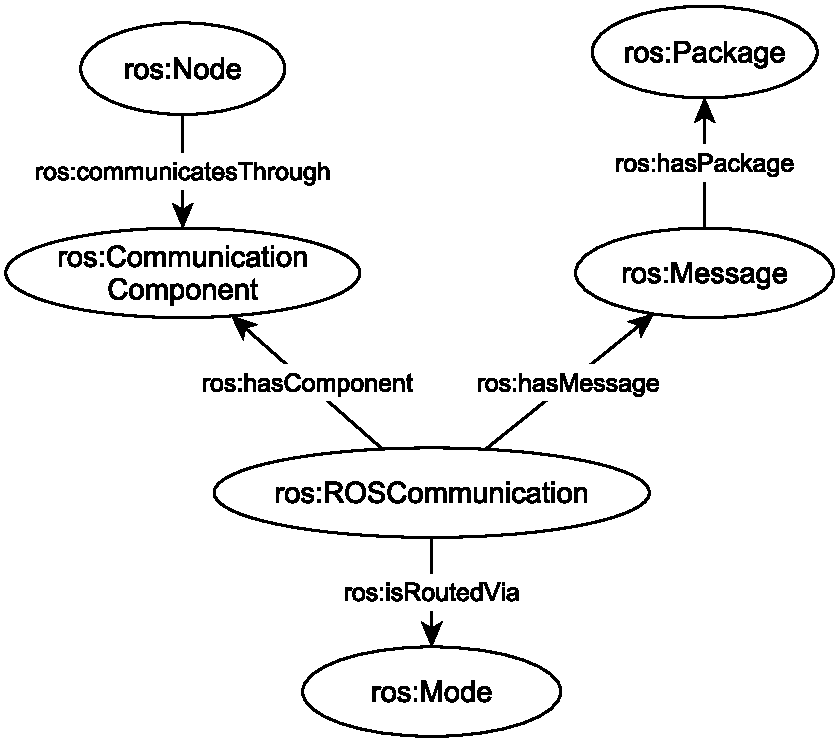
\includegraphics[width=.45\textwidth]{gfx/onto/basic}} 
    \subfloat[TODO]
    {\label{subfig:topic}%
    	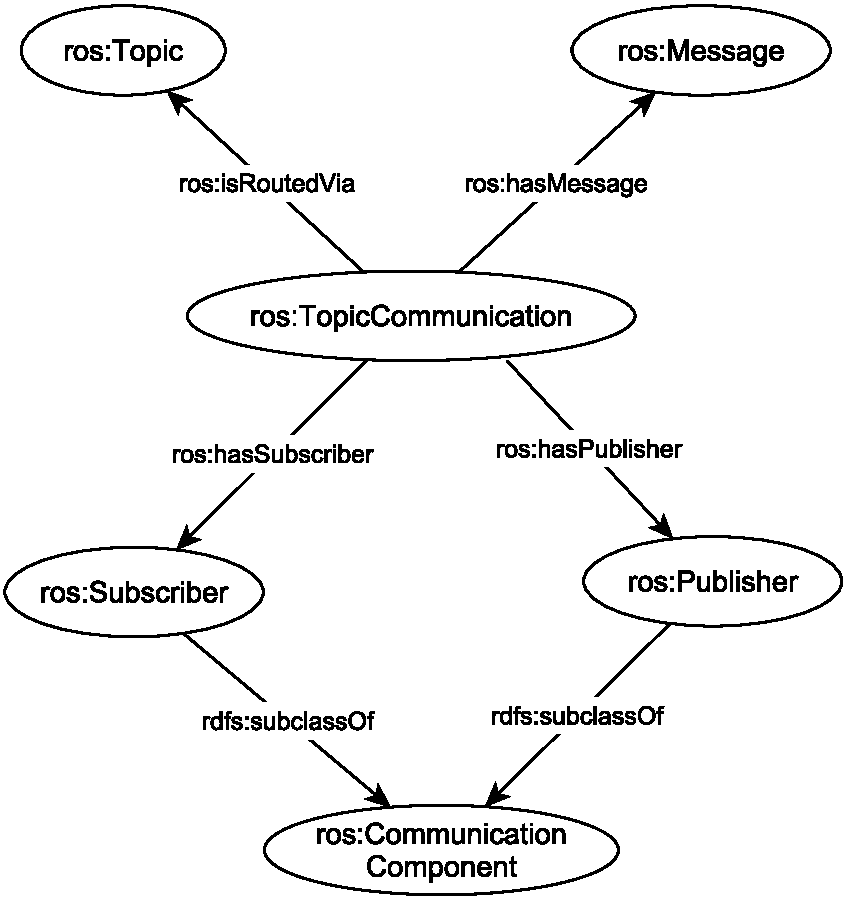
\includegraphics[width=.45\textwidth]{gfx/onto/topic}} \\
    \subfloat[TODO]
    {\label{subfig:service}%
    	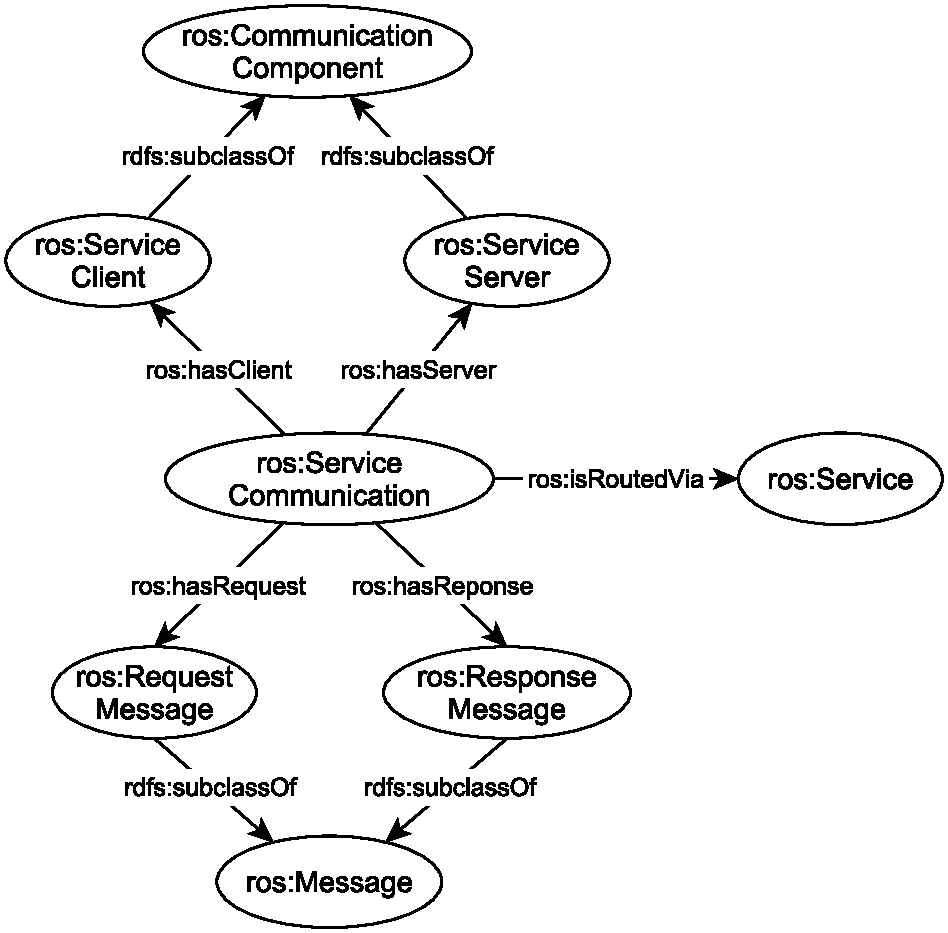
\includegraphics[width=.45\textwidth]{gfx/onto/service}}
    \caption[TODO]{TODO}\label{fig:ros-onto}
\end{figure}

\subsection{ROS description}
\label{sec:ros-desc}
Before the definition of robot capabilities it is necessary to create a formal representation described as an ontology of the main elements of ROS. While this is not used directly in the capability extraction process, it creates a structure that can be used as a reference and to contextualise the capabilities. Since the aim is not the creation of an ontological classification of ROS, but to define a framework for capabilities classification and extraction, we did not capture in the ontology every element of ROS. 

The final aim is to automatically extract which capabilities are exposed by a specific system, therefore, we can only exploit static information provided by the source code or dynamic information obtained from the runtime of the system. Given that ROS support various runtime-only configuration (\eg, topic remapping, parameters definition at start-up, dynamic reconfigure, \etc), we decided to focus on all the information obtainable when the system is running. In ROS, during runtime, the main source of information comes from the computational graph, a collection of all the active nodes and their connections. Various elements, other than nodes, are part of the graph, for example the ROS master or the parameters server, to build our ontology, we decided to focus only on those parts that are defined by the developer, both as a topology definition and as a complete implementation. In particular, we take in account:
\begin{itemize}
\item A \textit{node} is a process performing a specific computation and represent the minimal executable unit of ROS. A single node or a collection of nodes implement a specific functionality, therefore is connected to a potential capability of the robot.
\item \textit{Messages} are the typed data structure exchanged by the nodes when communicating with each other. Here we refer to messages in the broader sense, including all communication object exchanged in any type of communication. Messages are often generic (\eg, \textit{Vector3} in the \textit{geometry\_msgs} package), but when specific (\eg, \textit{Image} in the package \textit{sensor\_msgs})  they can be used to identify capabilities.
\item \textit{Topics} are the named channels used to exchange messages asynchronously using a publish/subscribe paradigm. Since they are completely user-defined, it is not possible to infer any significant information from them, however, they are fundamental to categorise capability, especially if multiple instances of the same one are available (\eg, multiple vision systems).
\item Similarly to topics, \textit{services} are named channels for synchronous communication, exchanging pairs of messages (\ie, request and response). Again, the service itself does not provide significant information since it is user-defined, however, it helps categorise the identified capabilities.  
\end{itemize}
While they are an alternative communication system between nodes, actions are not included in this analysis for multiple reasons. First of all, they are rarely used, therefore any extra effort to include them would provide little or no extra information. Additionally, given their complexity, they are, in most cases, completely defined by the developer and not based on any pre-defined message. Lastly, from a pure communication point of view, actions are only a collection of topics with a specific set of rules hidden to the developer by the action clients. 

Focusing on these elements we can define a formal representation of ROS and the interactions of its components. As said before, the aim of this ontology is to support the definition of the concept of capabilities and their automatic extraction from an existing system, therefore, while it is based on the Event and Situation ontology design patterns, it is not rigorously designed for robustness, completeness or originality. Figure~\ref{fig:ros-onto} show a graphical representation of the ontology describing the main ROS elements (Figure~\ref{subfig:basic}), and a more detailed description of topics (Figure~\ref{subfig:topic}) and services (Figure~\ref{subfig:service}).

\paragraph{Basic ROS description} Figure~\ref{subfig:basic} capture the main elements of ROS and how they are conceptually interconnected. ROS revolves around the concept of the computational graph, where nodes (\ie, executable components) are connected to each other through different type of communications (\ie, topics and services). Messages are the main carrier of information between different components. In ROS, there is one way to loosely aggregate elements by functionalities: packages. Nodes and messages have an assigned package, which is user defined, therefore not all of them are a reliable source of information to define the expected functionalities of an element. Nevertheless, some effort to create standard packages exists, some examples are \textit{sensor\_msgs} for messages used to encode sensor measurements, or \textit{navigation} for the planning, mapping and control nodes.

All these details are codified by the ontology. \textit{ros:Node} and \textit{ros:Message} are defined as part of a specific \textit{ros:Package}. The edges of the computational graph are identified by the \textit{ros:ROS\-Com\-mu\-ni\-ca\-tion} class, multiple relations exists between this class and the rest of the ontology. To identify the type of communication, we use the \textit{ros:Mode} class and the relation \textit{ros:isRoutedVia}, together they specify if a pair of nodes use an asynchronous (\ie, topic-based) or synchronous (\ie, service-based) communication system. The relation between \textit{ros:Node} and \textit{ros:ROS\-Com\-mu\-ni\-ca\-tion} is not direct, but it is mediated by a \textit{ros:Communication Component}. This class represent the interface implemented by the node to use a specific communication pattern, moreover, it is important to define the direction of the communication. For example, the a velocity message published by a single node and read by a multitude is more probably related by a speedometer, while multiple velocity publisher converging on a single subscriber can point to a set-point multiplexer.

This ontology was defined independently from the modelling approach defined in Chapter~\ref{ch:Modelling} and with no intention of establishing a encompassing definition. Nevertheless, there are recurring structures that appear both in the ontology and the  model. Clearly some are related to the internal structure of robotic middleware and frameworks, or mode in details to ROS itself. For example the definition of nodes (\ie, robotic components in the \textit{component-and-connector paradigm}) and messages (\ie, communication objects) appears in most component-based approaches. However, the necessity of specify a communication component acting as an interface between the the node and the communication system, is the same as the need to define AADL threads as a way to model the inner functioning of a component. In summary, it is never enough to just specify a components and its connection, it is necessary to detail the communication, its direction, the protocol, and the management system.

\paragraph{Topic description} Figure~\ref{subfig:topic} represents the extension of the previous ontology to better describe communication happening through topics. The central class of this ontology is \textit{ros:Topic\-Com\-mu\-ni\-ca\-tion}, which is a subclass of the more general \textit{ros:ROS\-Com\-mu\-ni\-ca\-tion}. Here we specify more in detail the protocol used by this type of communication by creating a subclass of \textit{ros:Mode} and defining \textit{ros:Topic}. The topic-based communication is the simplest protocol provided by ROS, implementing an asynchronous interaction based on the publish/subscribe protocol, additionally it uses a publish-and-forget approach. This is translated in the ontology by defining two subclasses for the communication component: \textit{ros:Subscriber}, as the subscriber of the protocol, in charge of receiving the messages, and \textit{ros:Publisher}, as the publisher, in charge of generating the messages. The lack of ownership of the messages and the absence of delivery confirmation result in a simple relation between the message and the topic.

To understand how an instance of a topic is defined with respect to the corresponding nodes, we  can take as an example a simple pair of nodes implementing a local planner feeding a control system with velocity set-points. They are connected by a named topic (\texttt{/cmd\_vel}) and exchange a specific type of message (\textit{geometry\_msgs/Twist}). The local planner implements a publisher, while the control system implements a subscriber. The resulting representation is in Listing~\ref{lst:onto-topic}.

\begin{lstlisting}[frame=tb,caption={TODO},label=lst:onto-topic]
@prefix ros: <onto-ros/class#>
@prefix : <onto-ros/resource/>
:setpoints a ros:TopicCommunication;
	ros:isRoutedVia :cmd_vel;
	ros:hasMessage :twist;
	ros:hasPublisher :cmd-output;
	ros:hasSubscriber :cmd-input.
:twist a ros:Message.
:cmd-vel a ros:Topic.  
:local-planner a ros:Node;
	ros:hasComponent :cmd-output.
:controller a ros:Node;
	ros:hasComponent :cmd-input.
 \end{lstlisting}

\paragraph{Service description} Figure~\ref{subfig:service} represent a second extension of the basic ontology to describe the synchronous communication approach provided by services.  As for topics, the central class is \textit{ros:Service\-Com\-mu\-ni\-ca\-tion} as a subclass of \textit{ros:ROS\-Com\-mu\-ni\-ca\-tion}. To identify the protocol implemented by services, we created a dedicated subclass of \textit{ros:Mode} called \textit{ros:Service}. Given their
synchronous approach, messages exchanged during the execution of a service are divided in two categories: requests, sent by the client to trigger the functionality provided by the service, and response, sent by the server with the result of the computation or as a completion notification. To capture this we defined two subclasses of the original \textit{ros:Message}: \textit{ros:Request Message} used to classify the request sent by the client, and \textit{ros:Response Message} used to identify the response sent by the server. As for the topic, it is necessary to specify, using subclasses of \textit{ros:Communication Component}, the specific interfaces implemented by the node when acting as a client or as a server. The two subclasses are: \textit{ros:Service Client}, for the client, and \textit{ros:Service Server}, for the server.

Listing~\ref{lst:onto-service} provides a small example on how an instance of a service is represented using the ontology. In the example there is a global planner that needs to synchronously request an occupancy grid from the map server. They interact using a named channel (\texttt{/map}), the client (\ie, the global planner) send an empty message (\textit{std\_msgs/Empty}) as a request to the server (\ie, the map server) to trigger the delivery of the map through the response (\textit{nav\_msgs/OccupancyGrid}). Each node, depending on its role, implements a service client or a service server.

\begin{lstlisting}[frame=tb,caption={TODO},label=lst:onto-service]
@prefix ros: <onto-ros/class#>
@prefix : <onto-ros/resource/>
:map-service a ros:ServiceCommunication;
       ros:isRoutedVia :map;
       ros:hasMessage :occupancy-grid;
       ros:hasClient :map-request;
       ros:hasServer :map-response.
:occupancy-grid a ros:Message.
:map a ros:Service.  
:global-planner a ros:Node;
       ros:hasComponent :map-request.
:map-server a ros:Node;
       ros:hasComponent :map-response.
 \end{lstlisting}
 
\subsection{Capabilities extraction}
\label{sec:cap-ext}
The ontology defined in Figure~\ref{fig:ros-onto} is useful to understand the most significant and recurrent elements of a ROS-based system. The main insight is the recurring relationship between a node, a message and a specific communication pattern (\ie, service or topic). These three elements together can be used to identify high-level capabilities of the robot and potential entry points.

To better understand how this triple (\ie, node, message, and communication patter) can identify a capability, we can recall the examples described in the previous section. Let us start by analysing the pair nodes involved in a simple control subsystem. On one side, there is the local planner, it uses a publisher to generate a \textit{Twist} message on the \texttt{/cmd\_vel} topic. We cannot extract significant knowledge from the node itself, except for the fact that it implements a publisher, therefore we can infer the direction of the communication. Since \textit{Twist} is one of the standardised messages, we know that is commonly used to exchange set-points (speed sensor usually rely on \textit{Odometry}), hence we can conclude that this specific message published by the node on a specific topic can be read to have an insight on the expected velocity of the robot. On the opposite side of the topic there is the control node. Since they are connected directly, it shares the same type of message (\ie, \textit{Twist}) and the same topic (\ie, \texttt{/cmd\_vel}) of the local planner. However, the control node implements a subscriber, this changes completely the meaning of the message. While the assumption that \textit{Twist} is used for set-points still stands, the different direction of the communication (\ie, from the topic to the node) let us know that we can use this message on this topic to control the movement of the robot.

A similar analysis can be done for the second example involving services. This pair of nodes implements a global planner requesting a map from the map server. On the provider side there is the map server, it implements a service server and advertises it with the name \texttt{/map}. As before, the named channel is completely user-defined, therefore there is no knowledge we can extract from it. From the node, since it implements the server, we can infer the direction of the communication: the map server receive the request and provide the response. On the receiver side there is the global planner, it accesses the service advertised by the map server using a service client. By this communication interface we can infer that the global planner will start the communication exchange. In the synchronous protocol of the service, two message are involved in the communication, in this case the request is an \textit{Empty} message, and the response is an \textit{OccupancyGrid} message. Since they are standardised messages, we already know to which functionalities they are usually related. An \textit{Empty} message carries no information, hence it can only be used as a trigger to activate another functionality. \textit{OccupancyGrid} is the standard message to share a bidimensional cell-based map where each cell can have three possible values (\ie, free space, obstacle or unknown), therefore we can easily assume that the result of this message will be a map of the environment. In summary, we can infer that both nodes support a map representation, the map server as the provider, hence we can trigger the service to receive a map, and the global planner as the receiver, this means we can setup a compatible service to impose a map to the planner.

By analysing these two examples, we can infer that establishing the mapping between a ROS-based system and the capabilities offered by the corresponding robot is equivalent to establishing a relation between a capability and a triple created by a node interface, a message and a communication protocol. In practice, there are four types of triples that we can define, that are a specialization of \texttt{<ros:Communication Component, ros:Message, ros:Mode>}:
\begin{itemize}
\item \texttt{<ros:Publisher, ros:Message, ros:Topic>} \\ This triple represents a capability evoked by an asynchronous communication. Since it is a publisher, it is possible to exploit it to interact with the system (\eg, teleoperation).
\item \texttt{<ros:Subscriber, ros:Message, ros:Topic>} \\ Similar to the one before, this capability is tied to an asynchronous channel. However, since it is evoked by a subscriber, it can be used to receive information from the system (\eg, sensing).
\item \texttt{<ros:Client, ros:Request, ros:Service>} \\ This triple represents the relation between a client and the synchronous protocol. By abstracting the interface created by this communication, we can control the expected response and inject a specific data content in the system.
\item \texttt{<ros:Server, ros:Response, ros:Service>} \\ This is the opposite side of the service-based communication protocol. By knowing the interface of the server, we can trigger its functionalities independently from the architecture.
\end{itemize}

As said before, the final aim of this approach is to create a system to automatically extract the capabilities of an existing architecture. As a result, it is necessary to define strict and clear rules relating a specific element of the ROS system to a capability; unfortunately, most of the architectural components of ROS are defined by the developer. There is no direct relationship between functionalities and node implementing them, for example, \textit{move\_base} incorporates a global and local planner in the same node, but a developer could implement them separately. Moreover, topics are completely user defined, they can be renamed at deployment time, or duplicated, therefore there is no connection between the name of the topic and its functionality. Lastly, the use of messages is unrestricted, a very pedantic developer could decide to use only custom messages in his architecture. Thankfully, ROS provides a wide variety of already defined messages, and, through component reuse, a self-standardisation process emerged. For instance, a \textit{Pose} message from the \textit{geometry\_msgs} package will, most of the time, provide information about the pose of the robot in a tridimensional space.

\begin{figure}[t]
\centering
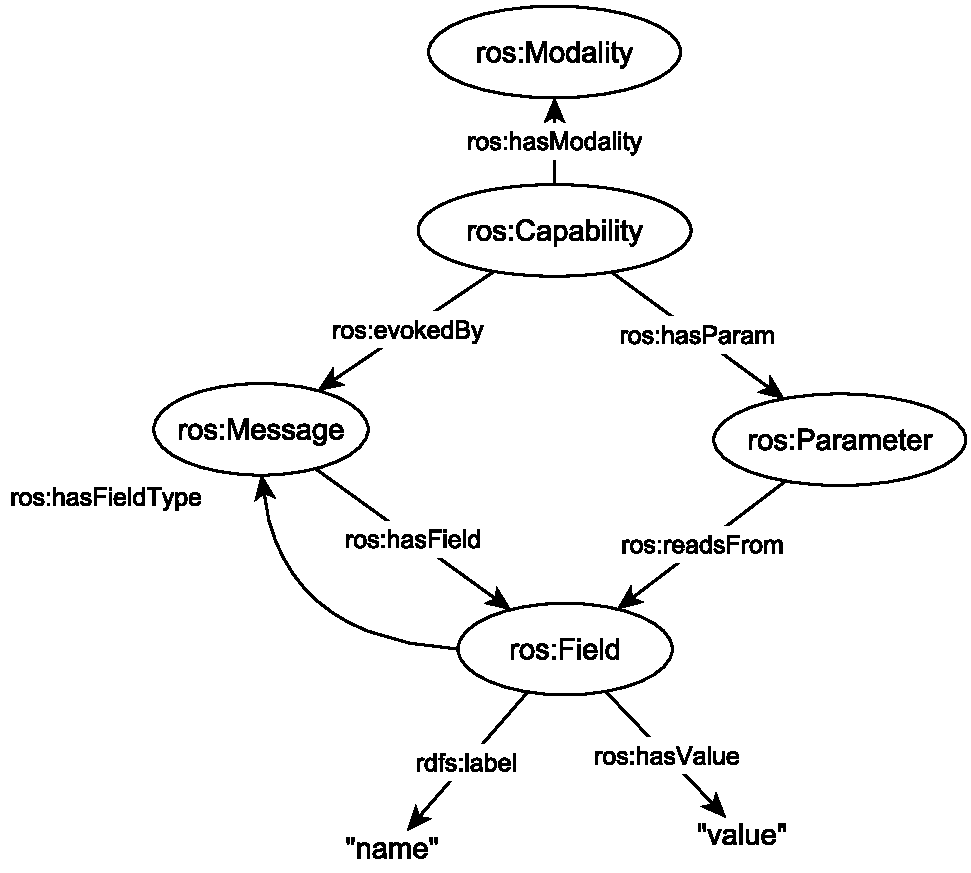
\includegraphics[width=0.70\textwidth]{gfx/onto/comptocapa}
\caption{TODO}
\label{fig:onto-capa}
\end{figure}

Given all these considerations, the resulting ontology to relate capabilities with portion of a given ROS architecture is presented in Figure~\ref{fig:onto-capa}. On the left hand side of the figure, we recall the three main elements related to a specific capability: message, communication component and mode. Since the only semi-standardised element of this triple is the message, a capability is evoked directly by a specific message. For instance, a \textit{LaserScan} message evokes the capability of sensing the environment using a laser sensor. Capabilities are characterised by a modality, they can be \textit{read} or \textit{write}. A capability has a \textit{read} modality when it can provides information to an external user, for example, collecting the map from the map server is a \textit{read} capability. The \textit{write} modality means an external user can influence the behaviour of the architecture, for example, teleoperation is a \textit{write} capability. The modality of a capability is defined by the type of communication component associated with it: publishers and servers are associated with \textit{read} capabilities, since an external user can collect information by reading their output, subscribers and clients evoke \textit{write} capabilities, it is possible to change the behaviour of a system by providing a specific input. In some cases capabilities express both \textit{read} and \textit{write} modalities. An example are all the sensing-related capabilities, an external user can read directly the output of a sensor or act as a sensor to change the behaviour of the system. In other cases only one modality is available, for instance, teleoperation is \textit{write}-only, because reading the joypad input is more related to sensing. The last part of the ontology is related to the application of the capabilities, the objective is not to just identify them, but to use them as an entry point for interacting with the robot. For this reason, each capability has a set of parameters, which are directly related to the fields of a message. A parameter can read from (or write to) a specific message field to create an instance of a message to interact with the robot architecture.

\subsection{Capabilities taxonomy}
In the previous sections, we defined the ontological superstructure necessary to formalise a ROS-based system (\ie, Figure~\ref{fig:ros-onto}), to define the relation between ROS elements and capabilities (\ie, Figure~\ref{fig:onto-capa}), and to extract capabilities from a running system (\ie, binding between messages and capabilities). This approach is completely general and not bound to any specific definition of the concept of capability other than \textit{``something the robot is capable of''}, it can be as high-level as \textit{``navigate to a goal''} or as low-level as \textit{``last fix of the GPS''}. However, to be able to apply this approach to a real robotic system, we defined a potential taxonomy of capabilities; the result is presented in Figure~\ref{fig:taxo}.

\begin{figure}[t]
    \myfloatalign
    \subfloat[TODO]
    {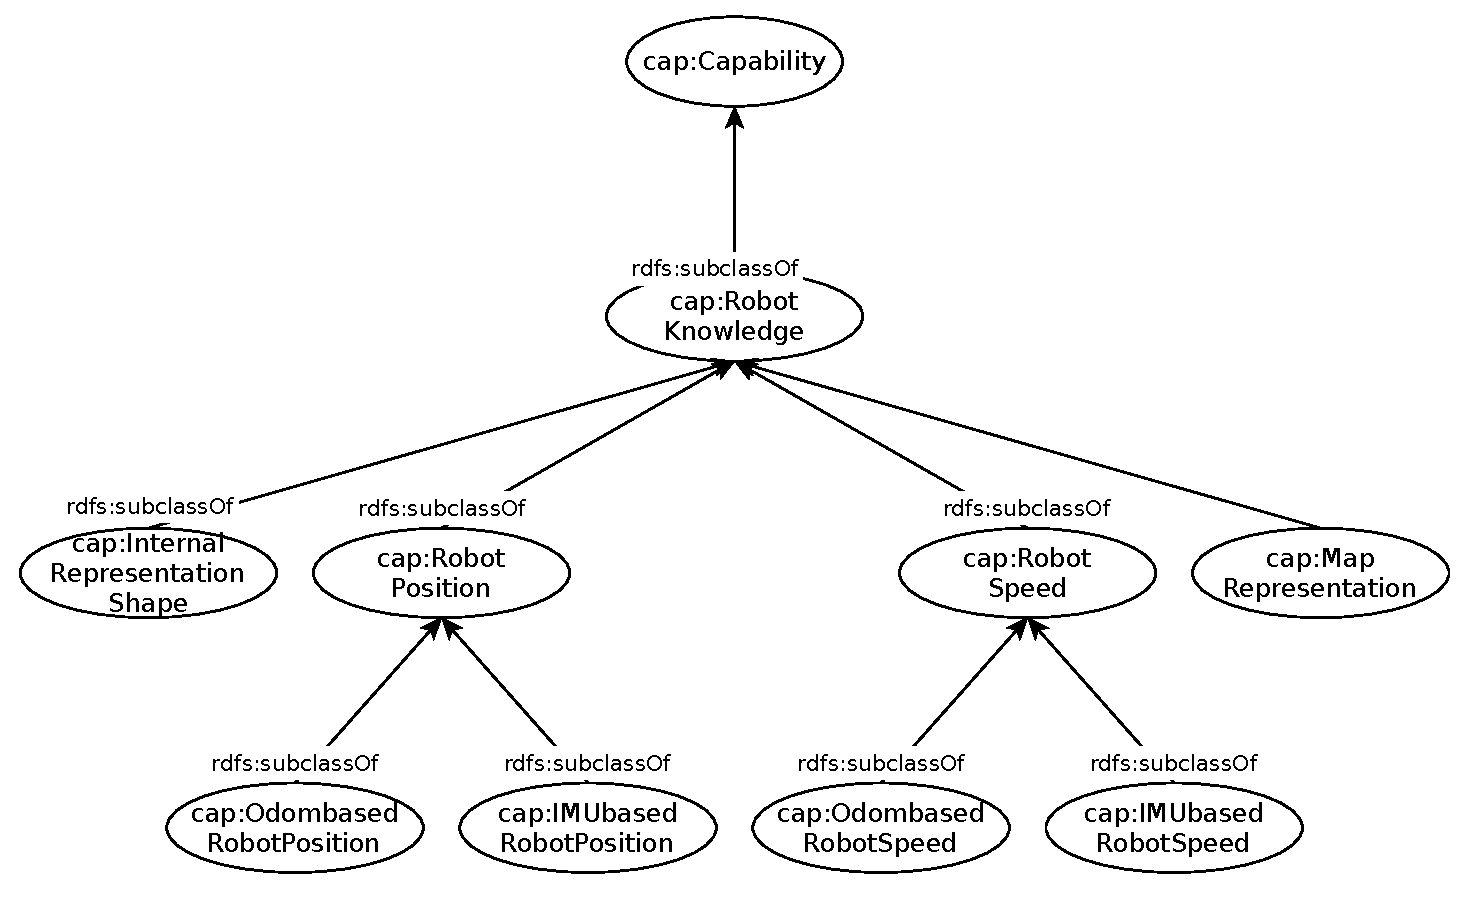
\includegraphics[width=.45\textwidth]{gfx/onto/taxo1}} 
    \subfloat[TODO]
    {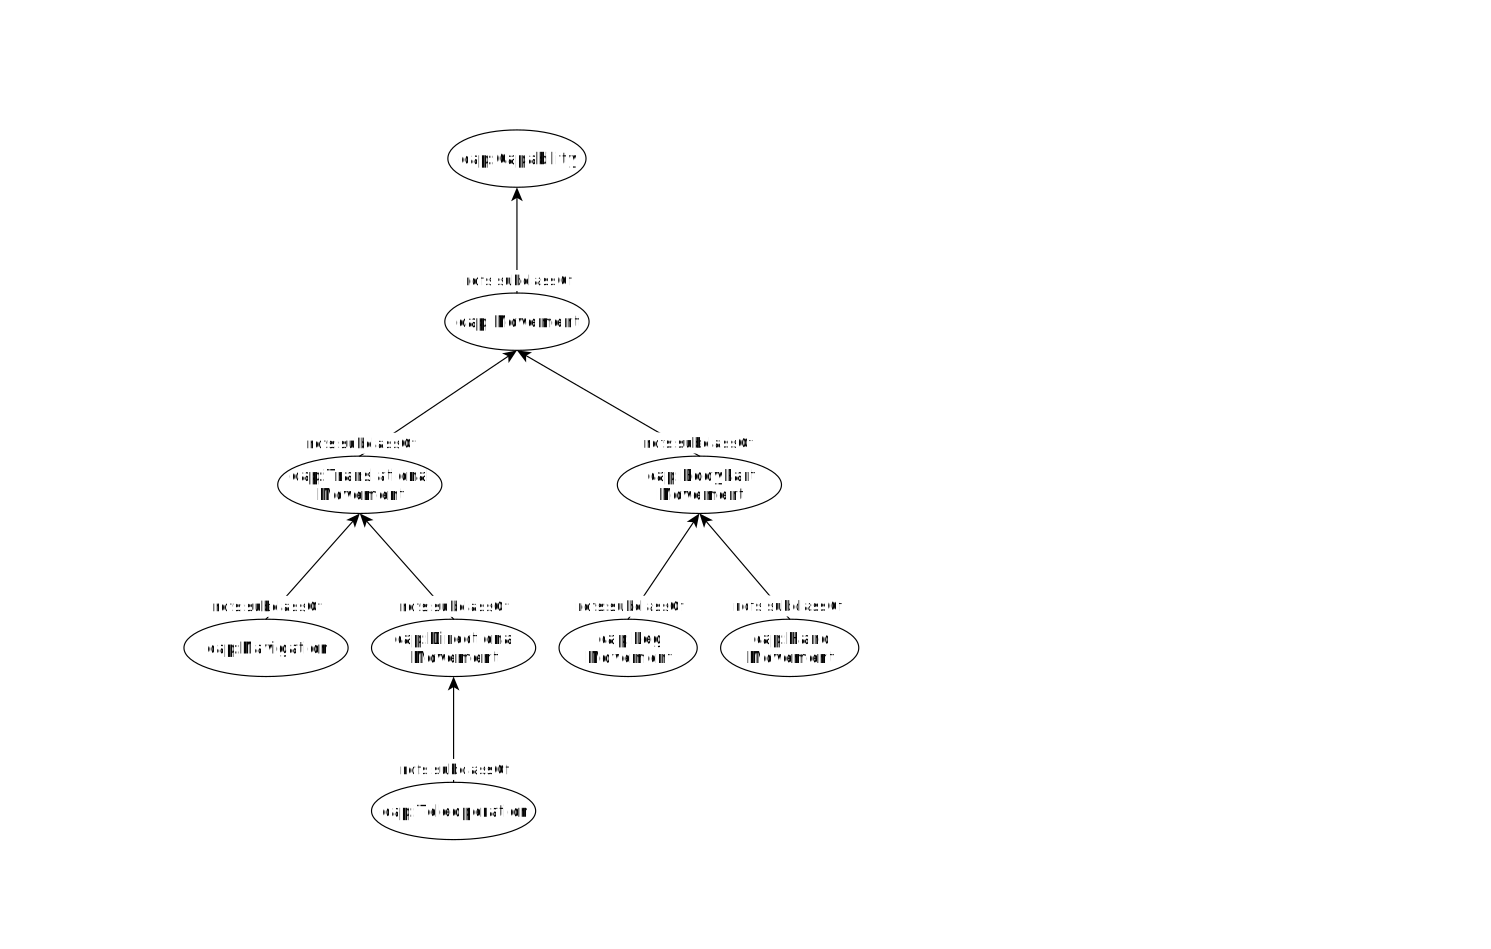
\includegraphics[width=.45\textwidth]{gfx/onto/taxo2}} \\
    \subfloat[TODO]
    {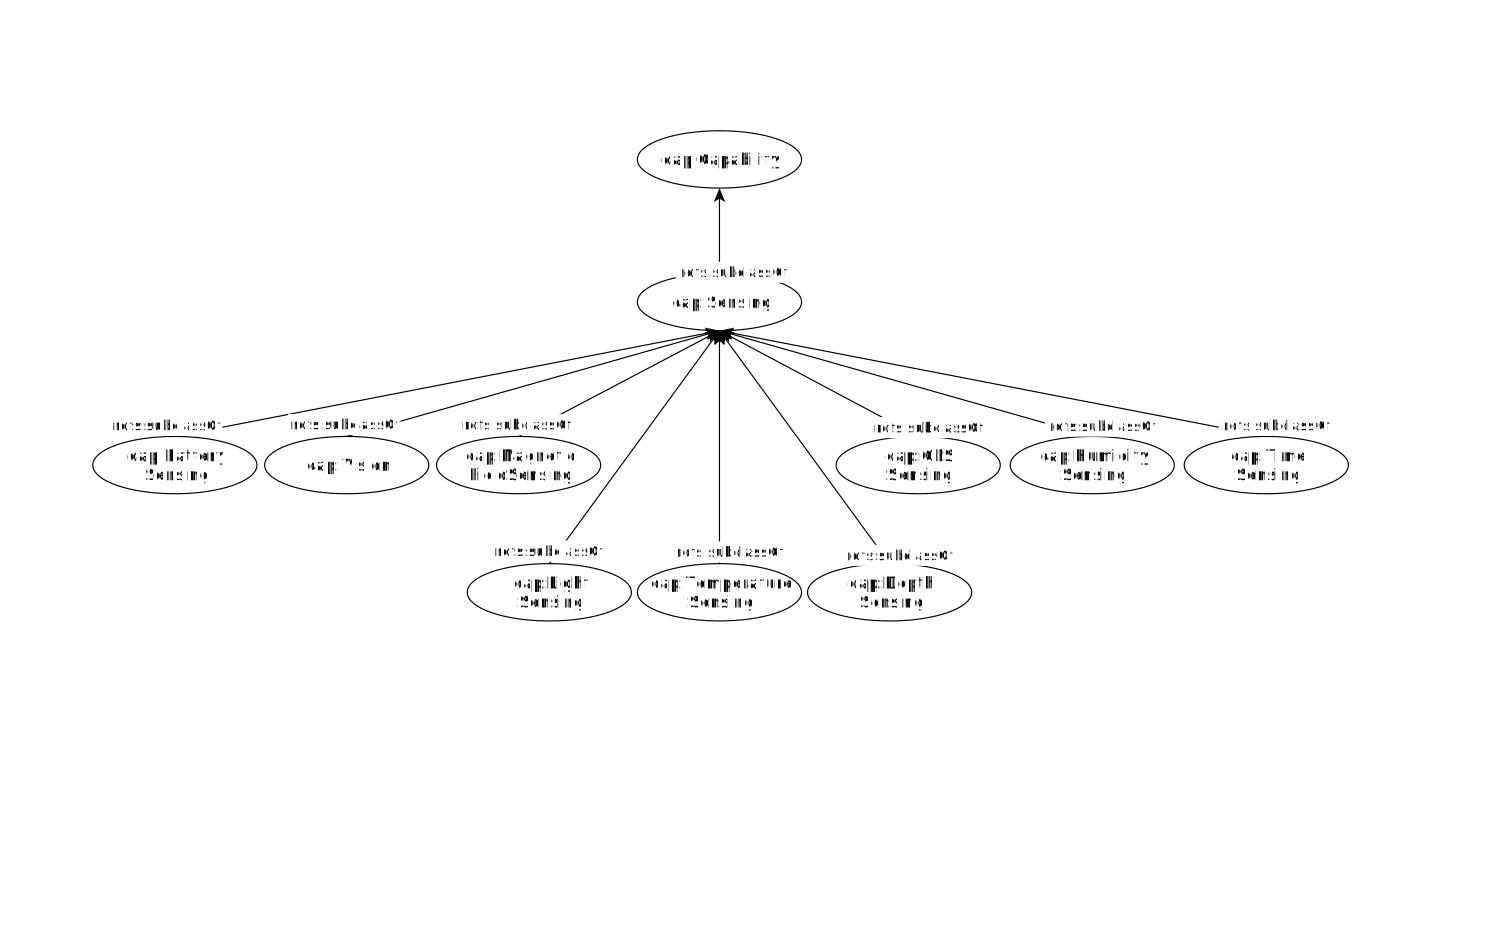
\includegraphics[width=.80\textwidth]{gfx/onto/taxo3}}
    \caption[TODO]{TODO}\label{fig:taxo}
\end{figure}

The root of the taxonomy is a general unspecified capability. From this there are three possible subclasses: sensing, robot knowledge, and acting. These three subclasses are meant to recall the \textit{sense-plan-act} paradigm, and focus on the three main characteristics of a robot: the ability of understand the environment through sensor, the ability of process the inputs and represent them, and the ability to interact with the environment through actuators.

In the \textit{cap:Sensing} subclass there are capabilities covering different type of sensing, both for perception (\eg, \textit{cap:Vision}) and proprioception (\eg, \textit{cap:Battery}). In this taxonomy, the sensing capabilities are directly connected to a specific sensor (\eg, a magnetometer for \textit{cap:Magnetic Field}), however, under this macro-category it is possible to fit capabilities obtained after one or multiple processing steps, if they provide direct information about the environment. For instance, AR tags detection could be a \textit{cap:Sensing} capability, since it provides the position of a particular object in space after processing an image. It is difficult to define the frontier where an input has received enough processing to lose the status of sensing, an option is to consider the need of external knowledge.  A GPS driver process an input stream using a standardised process, therefore is sensing, however, estimating the position of the robot from a velocity measurement requires specific information about the kinematic of the robot, hence it cannot be sensing.

In the \textit{cap:Robot Knowledge} subclass fall all those capabilities that are related to any internal representation used by the robot (\eg, \textit{cap:Map representation}), or any intermediate processing done to achieve the interaction with the environment (\eg, \textit{cap:Gobal planning}). This is potentially the largest subclass, since it encompass anything in between the sensors and the actuators, this is done on purpose, since it is difficult to categorise the functionality of a robot. In our version of the taxonomy, we mostly focus on mobile navigation, by including capabilities related to the robot position, the mapping of the environment and the physical shape of the robot. Most of these capabilities may not be relevant for a different type of robot, for example a manipulator may include object classification, grasping configuration estimation or inverse kinematic.

The \textit{cap:Acting} subclass may be the simplest to define, any capability that cause an action of the robot falls here. Any direct or indirect interaction with the environment, or change of configuration of the robot can be considered part of the \textit{cap:Acting} subclass. Again, we focus mostly on mobile navigation, therefore our taxonomy includes movement-related capabilities, like \textit{cap:Navigation} or \textit{cap:Teleoperation}. However, any other form of interaction can be categorized in this subclass, for instance, speech, grasping or visualisation (\eg, a robot equipped with an onboard tablet).

\section{Robot APIs} 
A formal definition of robot capabilities (functionalities, actions, tasks, \etc) is a topic often discussed, but very difficult to frame and resolve. We do not have the audacity of suggesting that our approach is the only possible solution, and more importantly, we know for sure that the taxonomy we presented is far from being exhaustive. However, our aim was never to provide the definitive classification for robot capabilities, it was a more practical one: to create an abstraction layer between the functionalities provided by modern robotic middleware and a potential \textit{application developer}. What we want to achieve is to view the robot architecture as a whole, a system providing a set of entry points that a developer can use to create high-level applications exploiting the capabilities of the robot.

The motivating scenario that pushed us in the direction of considering robotic platforms as abstracted entities providing a common interface is the integration of robots in smart-cities. Milton Keynes is a city in Buckinghamshire, England, that engaged in a series of programs to develop a ``Future City''. One of this was the MK:Smart project, which has developed a state-of-the-art data acquisition and management infrastructure (the MK~Data~Hub) and an IoT network of sensors. The MK Data Hub was built with the idea that a common facility to efficiently manage, integrate and re-deliver data from a variety of sources could be exploited by applications and services, reducing their development costs and enabling intelligent data management (mining, analytics, aggregation, alignment, linking) at the scale of the entire city. Given this, it is just a short step to introduce robots as an additional actor in the network of sensors connected to the smart-city; to integrate them as as data collectors~\cite{tiddi2016update} and data consumers~\cite{daga2016addressing}.

To better clarify the role of robots in the smart-city as actors of the integrated data acquisition and management infrastructure, we can provide a simple example. In Milton Keynes, a door-to-door robot-based delivery system is currently active. These robots travel around the cycle paths to deliver grocery upon request and are equipped with various sensors including cameras. At this moment, the information collected by the robot during their deliveries is not used for any additional task, but by integrating them in a larger system they could use their cameras to spot abandoned garbage on the cycle path. Of course, the delivery robot itself cannot pick up the trash, but it can notify the centralised data system about its discovery, the system will then aggregate all the information and setup a path for a garbage collector robot to clean up the cycle path.

With the current technology landscape for robotics this application would require the development of a series of ad hoc interfaces between each of the robot involved and the centralised data management system. In the particular example presented there is the additional complication that the delivery robots are owned by a private company, which is not keen to disclose the internal functioning of its machines.  All these problems can be resolved by introducing an abstraction layer. 

In this section, we present all the necessary tools we developed to create a set of robot APIs based on our definition of capabilities that can be used to completely abstract a ROS-based architecture. Figure~\ref{fig:robot-api} shows an overview of the complete system. Some elements are ROS-bound and are used to setup the abstraction layer, others are independent from the architecture and define the agnostic APIs to interact with the robot.

\begin{figure}[t]
    \centering
    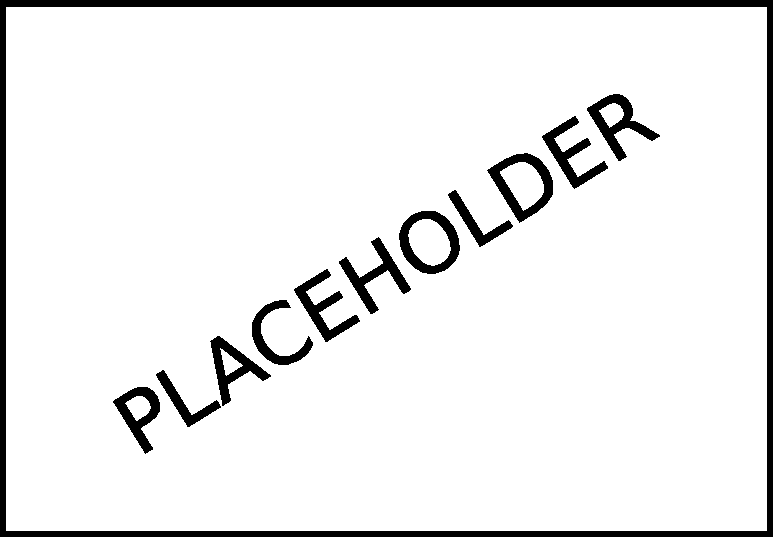
\includegraphics[width=0.8\textwidth]{gfx/placeholder}
    \caption{TODO}\label{fig:robot-api}
\end{figure}

\subsection{ROS-bound interface}
Figure~\ref{fig:robot-api} presents the complete set of elements necessary to interact with the robot. Three of them are enclosed in a container labelled \textit{ROS}. The reason of this distinction is because those three elements require a ROS-enabled environment to work. The first one is, reasonably, the robot, the collection of all the software and hardware components necessary to implement the functionalities provided by the system. There is no required on the structure of the architecture to be compatible with our approach, any ROS-based robot can be used. The only caveat is that our process, as described in Section~\ref{sec:cap-ext}, is based on the assumption that some specific ROS messages are used as expected from their semantic (\eg, \textit{Twist} is used for velocity). Directly connected to the robot, there is the \textit{Analyzer} and the \textit{Dynamic node}.

\paragraph{Analyzer} Before being able to interact with the robot, it is necessary to identify which functionalities it implements. In this initial phase is where the capability ontology described in Section~\ref{sec:onto} is used. While defining the relation between capabilities and ROS elements we highlighted how a capability evoked and specified by three elements: communication interfaces, messages and communication channels. The role of the \textit{Analyzer} is to use a list of binding between message types and capabilities to create a knowledge base containing all the available functionalities of a specific robotic platform.

Thanks to the effort spent in defining the ontology, the process of extracting the capabilities is quite straightforward. First of all, it is necessary to start the complete robot architecture, when all the nodes are up and running, we can run the \textit{Analyzer}. The \textit{Analyzer} loads a list of message/capability binding, then analyse the entire computational graph of the target ROS architecture. For each topic or service and their associated communication interface (\ie, publishers and subscribers for topic, client and servers for services), the \textit{Analyzer} adds an entry in the knowledge base. Each entry create a relationship between a communication channel and a specific capability through a message. Recalling the example of the controller introduced in Section~\ref{sec:ros-desc}, the entry in the knowledge base would create a relation between the \texttt{/cmd\_vel} topic, the \textit{Directional Movement} \textit{write}-capability and the \textit{Twist} message.

A significant upside of creating a knowledge base instead of using a runtime approach is that the output of the \textit{Analyzer} is permanent. If the architecture does not changer, there is no need to run the component again. This means that robots with the same architecture shares the same capability knowledge base, and that a single knowledge base can be created at deployment-time and shipped together with the architecture of the robot.

\paragraph{Dynamic node} Together with the definition of the capabilities, there is another element necessary to correctly implement an API system: a reliable interface with the ROS architecture. Given the structure of the ROS computational graph (\ie, communication channels supporting an \textit{n-to-n} cardinality), it is not difficult to inject or read messages from the architecture. In fact, ROS itself provides various tools to interact with the system at runtime (\eg, \texttt{rostopic} and \texttt{rosnode} family of commands). However, most of these commands are meant to be run from a terminal and designed for the occasional interaction, hence are not suitable to be used as a unified interface between the robot and an external system.

For these reasons, we implemented the \textit{Dynamic node}; its role in the API system is as simple as it is crucial. It relays the interaction coming from capability-based environment of the external user to the ROS-enable environment of the robot by acting as a frontier between the two. The \textit{Dynamic node} implements a system to create and destroy dynamically the suitable communication interfaces associated with a specific capability. To better clarify, let us take again the example of the velocity controller. From the \textit{Analyzer} we know that the node exposes a subscriber to the topic \texttt{/cmd\_vel} and the message exchanged is \textit{Twist}. The \textit{Dynamic node} can use these information to dynamically create a publisher on the specified topic with the specified messages, and then, upon request, publish content on the topic.

In order to make the approach more general, the \textit{Dynamic node} does not require the content of the message to be defined as an actual ROS message. It expects a Python dictionary with the same structure of the message. Moreover, it supports multiple form of communication: one-shot interactions with the topics (\ie, publish or read a single message), complete bidirectional relay of messages, and client and server replacement. The {Dynamic node} is developed for generality, while the superstructure provided by the capabilities makes the interaction easier, it can be used directly as a dynamic interface to the architecture. In summary, it provides a semi-agnostic (\ie, it requires a ROS-enabled environment to run and the knowledge about topics and messages) local API to interact with a ROS-based system.

\subsection{ROS-independent interface}
By going back to Figure~\ref{fig:robot-api}, it is possible to see that no other element is inside the \textit{ROS} container. This means that the rest of the system is completely ROS-independent and can be run on any platform. The way we structured the APIs is guided by the smart-city and robot interaction scenario. What we wanted to achieve was to define an interaction approach that a remote data management system can use to receive information from the robot and send commands and instruction without having to implement any ROS-related (or, more in general, robotic-related) interface. By following these specifications, we developer a \textit{Server} and, finally, the \textit{OntoRob Interface}. Of course this approach can altered by removing the \textit{Server} and integrating some of its functionalities in the \textit{OntoRob Interface}; the result is moving from a remote APIs approach to a local one.

\paragraph{Server} The role of the \textit{Server} is to create a completely ROS-agnostic interface to the robot. Differently from the \textit{Dynamic node}, not only the the structure of the messages is not related to ROS, but also there is the shift from the \textit{node/message/topic} paradigm, to \textit{modality/capability/parameter}. In summary, the \textit{Server} is the capability-centric interface to the robot.

The \textit{Server} provides a list of remote APIs that can be called to receive information or interact with the target system. Since it has access to the knowledge base it can provides the list of the active capability with their corresponding topic/service name. In this case, the name is only an identifier, since the same capability can appear multiple times in a system (\eg, two \textit{Vision} capabilities from stereo cameras), we need a way to identify them. As described in Section~\ref{sec:cap-ext}, each capability has a list of parameters that mirrors the fields of a ROS message. These information can be used to activate the \texttt{/read} and \texttt{/execute} APIs of the \textit{Server}.

During his normal execution, the \textit{Server} subscribes through the \textit{Dynamic node} to all the topics associated with \textit{read}-capabilities. When an external user triggers the \texttt{/read} API using a pair capability-topic, the \textit{Server} will first check in the knowledge base that the requested pair is legal, and then it will answer with the last messages exchanged on the topic, suitably converted using the parameters of that specific capability. With the opposite approach, when an external user triggers the \texttt{/execute} API, the \textit{Server} receive a triple composed by: a \textit{write}-capability, a topic name, and the parameters corresponding to that capability. As before, first the \textit{Server} checks for the command validity and then converts it to a suitable data structure to feed it to the \textit{Dynamic node}. To increase the flexibility and the generality of the interaction, all the exchanges between the external user and the \textit{Server} are done using JSON.

\paragraph{OntoRob Interface} In theory, the \textit{Server} provides a complete enough interface to remotely interact with the robot. It gives all the necessary capabilities, it provides the output of topics or services, and receives commands. A centralised data management system like the MK~Data~Hub that triggered the implementation of this approach would directly interact with the \textit{Server}. However, our long term vision was to develop a interface to support the development of robotic applications, hence we developed a Python-based that can be easily integrated in a computer program as a developer would do for any other API.

The \textit{OntoRob Interface} is a class that can be instantiated to establish a connection with \textit{Server} and hide the complexity of the JSON-based interaction. The class provides a more streamlined and compact interface that can be used to integrate the functionalities provided by the \textit{Server} in a Python program. It has method to obtain knowledge about the current active robotic system: the list of topic (as before, used as capability identifiers), the list of capabilities, the relation between the two, the structure of messages. Additionally to all these methods, it provides APIs to retrieve information from \textit{read}-capabilities and interact with the robot through \textit{write}-capabilities.

\begin{figure}[t]
    \centering
    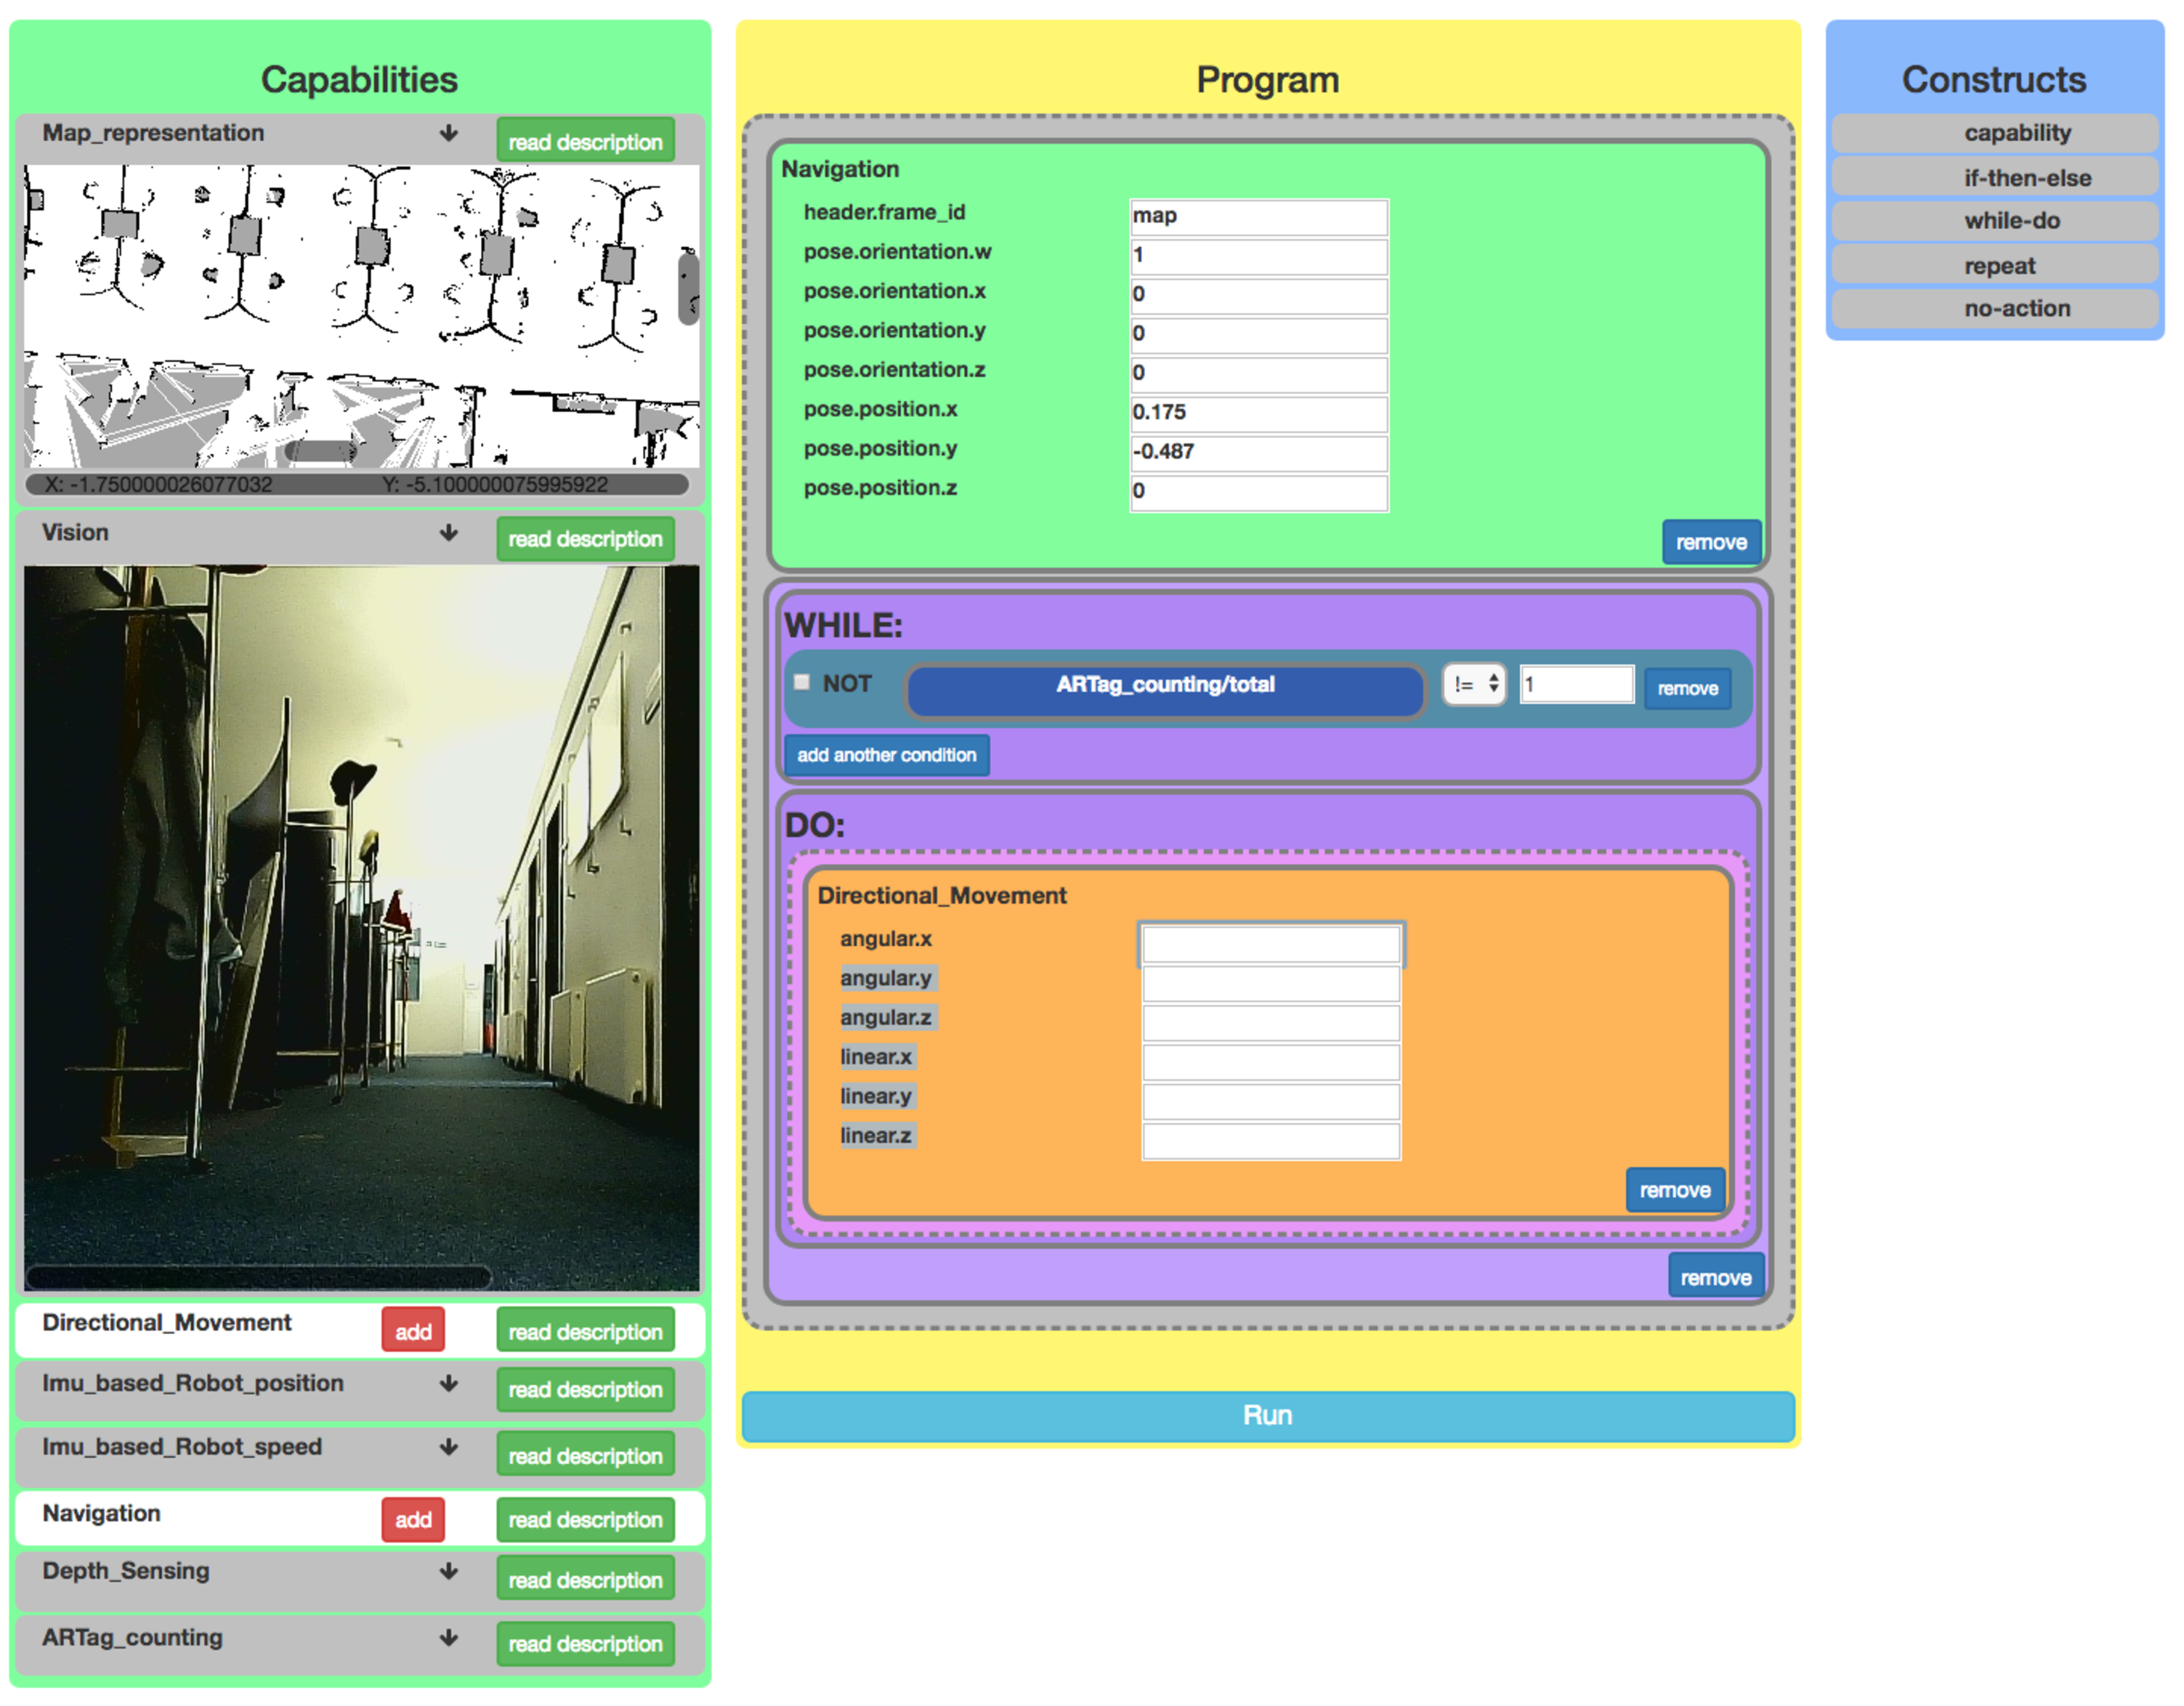
\includegraphics[width=0.9\textwidth]{gfx/onto/web}
    \caption{TODO}\label{fig:web-api}
\end{figure}

\section{Web interface}

\subsection{GUI description}

\paragraph{Capability Panel} This panel offers the users the list of capabilities abstracted from a robotic platform to which the system is connected. We refer the reader to~\cite{tiddi2017ontology} for the in-depth description of the ontology-based system lying behind the interface. Here, we limit ourselves in mentioning that the system is based on a formal representation of the ROS architecture (in short, \textit{:Node}s that exchange \textit{:Message}s routed via specific \textit{:Topic}s), and that such communication exchanges mapped into specific robot \textit{:Capability}(ies), organised into as a taxonomy whose highest classes are \textit{:Sensing}, \textit{:Movement} and \textit{:RobotKnowledge}. Based on the ontology and the robot running on ROS, an Analyser module scans all active ROS components to determine the capabilities processed by the robot, based on the high-to-low-level capability mappings described in the knowledge base.  The retrieved list of capabilities is then shown to the user, for he/she to create an ad-hoc program. Note that capabilities come in two modalities: \textit{read} capabilities, giving information about the robot (e.g. the \textit{Vision} capability offering data from a camera), and \textit{write} capabilities that expect some inputs (e.g. \textit{Navigation} expects a position in space). 

\paragraph{Construct Panel} The Construct Panel shows the user the set of  programming constructs that he/she can choose to create the program to instruct the robot with. A program can be created as an imperative programming language, in which the atomic blocks are invocations of the available robot capabilities on the left panel (using the \textit{add} button), and a set of conditional operators, such as \textit{if-then-else}, \textit{while-do} and the \textit{repeat} statement. An additional \textit{no-operation} statement can be employed to perform empty operations. The parameters of a capability can be used in the conditions, so to exploit any robot output to drive the program flow (e.g. moving forward until an object is detected). 
 
\paragraph{Program Panel} The Program Panel in the middle of Figure~\ref{fig:web-api} shows the user the program he/she has created through constructs and capabilities of the respective panels. Once the user is satisfied with the set of commands, they are sent to the robot through a Dynamic module. If a read capability is requested, the Dynamic module relays to the interface the messages received from the robot. If a write capability is requested, the Dynamic module reads the parameters from the interface, structures them in a message and then sends them to the robot, which consequently performs the operations.

\subsection{Experimental Setup}
 
Four exercises of increasing difficulty were asked to be performed by each user, which corresponded to creating a program allowing a robot to achieve a specific task. In order to demonstrate that the ontology-based system could allow the abstraction of robot capabilities independently from the platform, we set up two variants of each exercise, a simulated one with a ground wheeled robot operating in an office environment (\texttt{s}-variant), and a real-world one with a drone flying in an indoor space (\texttt{r}-variant). Table~\ref{tab:setting} presents the robot capabilities available in each setting\footnote{For clarity, autonomous navigation is related to the action ``go to a coordinate X,Y'', while directional movement is intended as commands such as ``turn right'' or ``move forward''.}.

\begin{table}[!ht]
\centering
\caption{Robot capabilities for the two exercise variants.}
\label{tab:setting}
\begin{tabular}{l|l|l}
\textbf{Mode} &\multicolumn{1}{c|}{\textbf{\texttt{s}-variant}} &\multicolumn{1}{c}{\textbf{\texttt{r}-variant}} \\ \hline
 & \multirow{2}{*}{autonomous navigation} & take-off  \\
write &\multirow{2}{*}{directional movement}& land \\
& &  directional movement \\ \hline

 & vision &  \\ 
 & current position & vision\\
read & current speed  & current position  \\
 & map representation & object recognition\\
 & object recognition 

\end{tabular}
\end{table}

\paragraph{Exercise~1: Single command.}  The first exercise required to implement a single movement behavior. In the \texttt{s}-variant, the user had to instruct the robot to move to a specific point in space corresponding to a room. Similarly, in the \texttt{r}-variant, the user had to instruct the drone with a single movement command.

\paragraph{Exercise~2: Command sequence.} In the second exercise, users needed to instruct a robot with a sequence of two single actions. In the \texttt{s}-variant, the users needed to instruct the robot to navigate to two rooms of the office, one after the other. In the \texttt{r}-variant, the user had to instruct the drone with any motion command, then ending its movement with a landing command. 

\paragraph{Exercise~3: Condition-based halt.} The third exercise required users to implement a sequence of actions with a termination condition. In the \texttt{s}-variant, the robot needed to perform a patrolling of three rooms of the office, stopping only once all the rooms had been visited at least twice. In the \texttt{r}-variant, the user had to instruct the drone to keep on turning on itself until an ARtag was seen, in which case it would land. 

\paragraph{Exercise~4: Object recognition.} In the final exercise, users had to instruct the robot to perform autonomous navigation through several ARtags. In the \texttt{s}-variant, the robot had to patrol a set of rooms until an ARtag was detected. In the \texttt{r}-variant, the user had to implement a behavior for the drone to perform 3 different movement actions every time an ARtag was seen.

\subsection{Results and discussion}

A total of 14 users were involved in the evaluation, equally shared between the \texttt{s}- and the \texttt{r}-variant. Those users were essentially members of our research lab with at least some basic programming skills (to make the exercise meaningful), but with no experience in either ROS or robotics in general. As a starting point, users were first allowed to familiarize themselves with the interface, namely through clicking on the different sections to understand the general behavior of the tool. Users were however prevented from reading the description of the capabilities. After this first step, they were  asked to solve all four exercises one after the other. For every exercise, we measured the time from the end of the task description until the final execution of the program. 

Table~\ref{tab:results} shows the average time \emph{avg}(\textsc{t}) required by the users to solve each exercise, along with the average number of programming blocks \emph{avg}(\textsc{pb}) and the number of capabilities \textit{num}(\textsc{cap}) required to solve the task.


\begin{table}[!ht]
\centering
\caption{Results for the \texttt{s}-variant and the \texttt{r}-variant. These are compared with the efforts required by a ROS expert to achieve the same tasks, measured in terms of number of lines of code \textit{num}(\textsc{ln}), ROS components \textit{num}(\textsc{com}) and ROS message types \textit{num}(\textsc{msg}) that were employed.}
\label{tab:results}
\resizebox{\linewidth}{!} {
\begin{tabular}{c|l|cccc}
\multicolumn{2}{l|}{} & Ex. 1 & Ex. 2 & Ex. 3 & Ex. 4 \\ \hline
\multicolumn{6}{c}{\texttt{s}-variant} \\ \hline
\multirow{3}{*}{\rotatebox[origin=c]{90}{users}} & \emph{avg}(\textsc{pb}) & 1     & 2     & 4     & 9.5   \\
& \textit{num}(\textsc{cap}) & 1     & 1     & 1     & 2     \\
& \emph{avg}(\textsc{t}) & 1:22 $\pm$ 42s & 1:04 $\pm$ 23s & 1:15 $\pm$ 16s & 6:52 $\pm$ 1:46 \\
\hline
\multirow{3}{*}{\rotatebox[origin=c]{90}{expert}} & \textit{num}(\textsc{ln})    & 35 & 58 & 64 & 82 \\
& \textit{num}(\textsc{com})    & 1 & 2 & 2 & 3 \\
& \textit{num}(\textsc{msg})    & 1 & 2 & 2 & 3 \\
\hline
\hline
\multicolumn{6}{c}{\texttt{r}-variant}                                     \\ \hline
\multirow{3}{*}{\rotatebox[origin=c]{90}{users}} & \emph{avg}(\textsc{pb})      & 1     & 2     & 4     & 8     \\
& \textit{num}(\textsc{cap}) & 1     & 2     & 4     & 4     \\
& \emph{avg}(\textsc{t})    & 1:16 $\pm$ 3s & 01:16 $\pm$ 8s & 4:05 $\pm$ 15s & 5:47 $\pm$ 1:39 \\
\hline
\multirow{3}{*}{\rotatebox[origin=c]{90}{expert}} & \textit{num}(\textsc{ln})    & 34 & 39 & 56 & 59 \\
& \textit{num}(\textsc{com})    & 1 & 2 & 4 & 4 \\
& \textit{num}(\textsc{msg})    & 1 & 2 & 3 & 3 
\end{tabular}
}
\end{table}

All the exercises were successfully carried out by all users. As one can see, Ex.~1 took slightly longer (especially in the \texttt{s}-variant), when compared with other more complex exercises. This can be attributed to the time users required to familiarize themselves with the capabilities of the robot they were working with, which they could not have known beforehand. The relatively high variance in the time taken for Ex.~4 is due to this particular exercise having multiple solutions, some of which taking longer to implement than others. 

A key, straightforward conclusion from this table is that users of this tool, who had no experience of programming robots and no prior knowledge of the architecture of the robot they were manipulating, managed to successfully program such a robot to achieve tasks from the very simple Ex.~1 to the more difficult Ex.~4 in a matter of a few minutes. Considering the inherent complexity of robot programming and of understanding not only what a robot can do (what capabilities it possesses), but also how to use it (how to invoke those capabilities), this can be considered a non-trivial achievement. 

A direct comparison with how the same users would have achieved the same tasks without the tool provided is not feasible and would turn out to be meaningless. 
However, it appears a straightforward assumption that, those users not being familiar with ROS, the simple (in our tool) process to understand the different components of the robot, what they do and, crucially, how to invoke them, would require more than a few minutes by itself. 
ROS is a complex framework, requiring hours of practice to master. In addition, analyzing the computational graph of the specific robot to understand which topics and services are being be used (i.e. what the tool does through the ontology) is far from an easy task. A number of ROS nodes would need to be implemented from scratch to encapsulate the required functionalities, and managing the correct publishers and subscribers. Lastly, the nodes would need to be deployed and integrated with the robot architecture. Knowledge of specific packages (e.g. the { \small \texttt{move\_base}} node for autonomous navigation) is also required by some of the exercises. In other words, while a direct comparison could not have been performed, there is little doubt that significantly more effort would have been required to enable our non-expert users to achieve the same results with ROS, as it did with our tool.

As an additional point towards the validity of our claim that our tool reduces the effort required to exploit robots' capabilities and therefore make them more accessible, we asked an expert in robotics with extensive experience in ROS to achieve the same task. Once again, the objective here is not to compare the experts to the non-experts using two different frameworks, but to provide an intuitive understanding of the difficulty of realizing the tasks achieved by our users without our tool. In Table~\ref{tab:results}, we therefore show for each task in each variant:
\begin{itemize}
\item The number \textit{num}(\textsc{ln}) of lines of code used by the ROS expert, 
\item The number \textit{num}(\textsc{com}) of ROS communication components (publishers and subscribers) employed %, which constitute one of the fundamental bricks of the ROS implementation 
\item The number \textit{num}(\textsc{msg}) of message types used. 
\end{itemize}
% While this is a na\"{i}ve comparison, 
These metrics give an estimate of the effort required by a ROS developer to solve the specified tasks. Lines of code set a lower bound for the implementation time, while number of components and messages outline the complexity of the solution.

This comparison further show how programming a robot is made ``easier'' and, through abstracting capabilities from the technical aspects of their implementation, requires less complexity. Our approach and the associated tool therefore represent a viable solution to enable non-expert users to exploit robots in ways that were before only accessible to expert ROS programmers. 

%it shows the idea that our approach is a viable solution to relieve non-experts from the efforts required to use the ROS middleware and, more generally, the robotic system's low-level components. 

\section{Bridge models and capabilities}

%*****************************************
